\subsection{Hidden Markov Models}

Hidden Markov models describe time series that exhibit state-switching behaviour. They model an observed time series of length $T$, $\bfY = \{Y_t\}_{t=1}^T$ by assuming that each observation $Y_t$ is generated from an unobserved hidden state $X_t \in \{1,\ldots,N\}$. The sequence of all hidden states $\bfX = \{X_t\}_{t=1}^T$ is modelled as a Markov chain. The unconditional distribution of $X_1$ is denoted by the row-vector $\bfdelta = \begin{pmatrix} \delta^{(1)} & \cdots & \delta^{(N)} \end{pmatrix}$, where $\delta^{(i)} = \bbP(X_1 = i)$. Further, the distribution of $X_t$ given $X_{t-1}$ for $t = 2,\ldots,T$ is denoted by the $N$-by-$N$ transition probability matrix 
%
\begin{equation}
    \bfGamma_t = \begin{pmatrix} 
    \Gamma_t^{(1,1)} & \cdots & \Gamma_t^{(1,N)} \\
    \vdots & \ddots & \vdots \\
    \Gamma_t^{(N,1)} & \cdots & \Gamma_t^{(N,N)} \\
    \end{pmatrix},
\end{equation}
%
where $\Gamma_t^{(i,j)} = \bbP(X_t = j \mid X_{t-1} = i)$. For simplicity, I assume that $\bfGamma_t$ does not change over time (i.e. $\bfGamma_t = \bfGamma$ for all $t$) unless stated otherwise. 

Each observation $Y_t$ is a random variable, where $Y_t$ given all other observations $(\bfY \setminus \{Y_t\})$ and hidden states $(\bfX)$ depends only on $X_t$. If $X_t=i$, then the conditional density or probability mass function of $Y_t$ is $f^{(i)}(\cdot ; \theta^{(i)})$, where $\theta^{(i)}$ are the parameters describing the state-dependent distribution of $Y_t$. The collection of all state-dependent parameters is $\bftheta = \{\theta^{(i)}\}_{i=1}^N$. A fixed realization of $\bfY$ is denoted as $\bfy = \{y_t\}_{t=1}^T$ and has probability density function
%
\begin{equation}
    p(\bfy ~;~ \bfdelta,\bfGamma,\bftheta) = \bfdelta P(y_1;\bftheta) \prod_{t=2}^T \bfGamma P(y_t;\bftheta) \mathbf{1}^\top_N, 
    \label{eqn:HMM_like_marginal}
\end{equation}
%
where $\mathbf{1}_N$ is an $N$-dimensional row vector of ones and $P(y_t;\bftheta)$ is an $N \times N$ diagonal matrix with entry $(i,i)$ equal to $f^{(i)}(y_t; \theta^{(i)})$. Parameter estimation for HMMs often involves maximizing Equation (\ref{eqn:HMM_like_marginal}) with respect to $\bfdelta$, $\bfGamma$, and $\bftheta$. Figure \ref{fig:HMM} shows an HMM as a graphical model. For a more complete introduction to HMMs, see \citet{Zucchini:2016}. 

\begin{figure}%[ht]
    \centering
    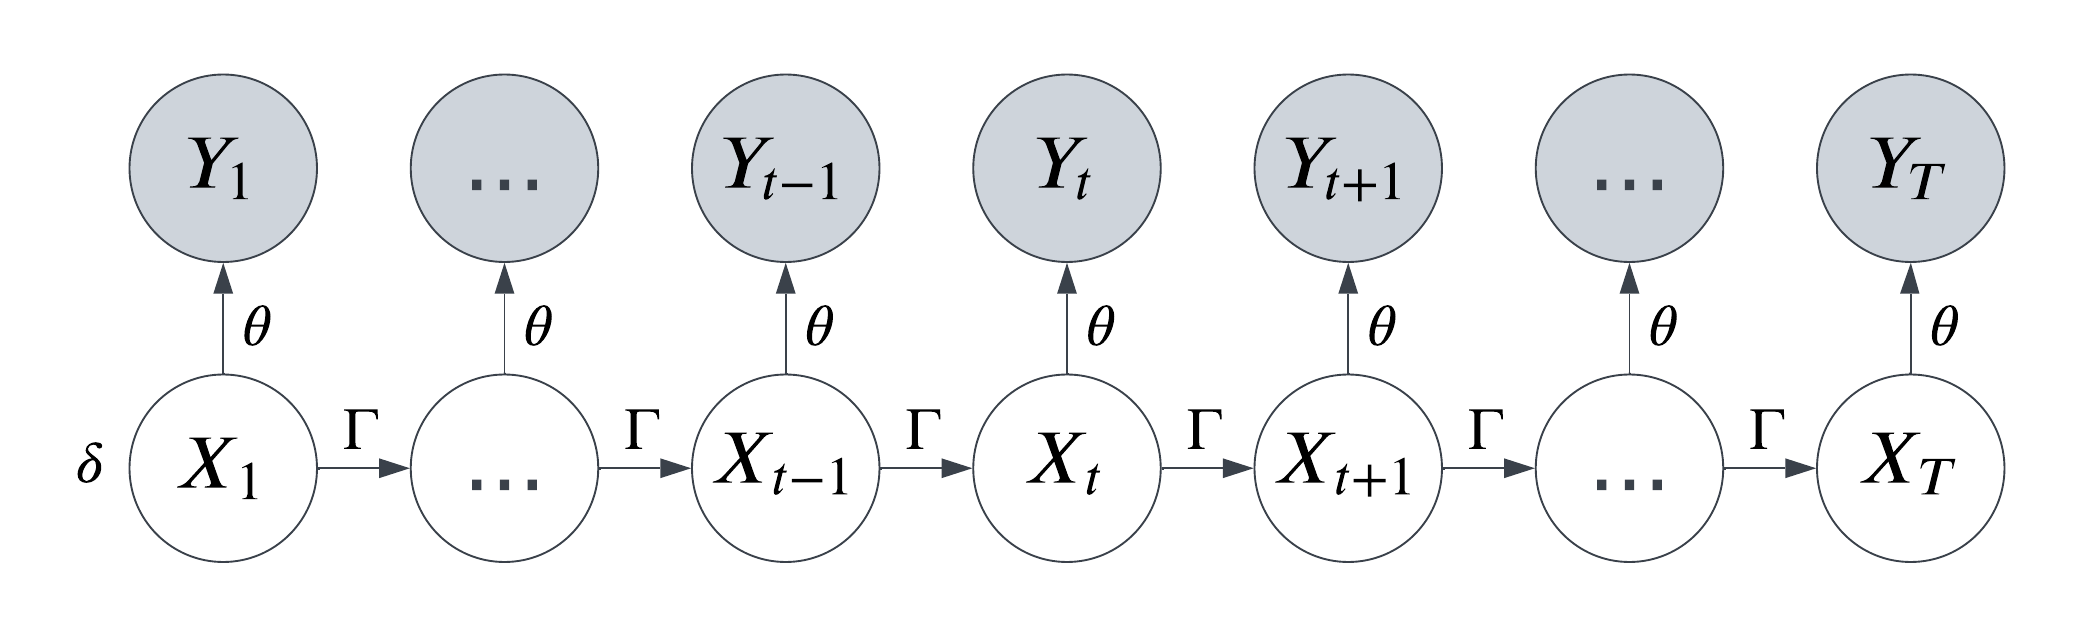
\includegraphics[width=5in]{../plt/HMM.png}
    \caption{Graphical representation of an HMM. $X_t$ corresponds to an unobserved latent state at time $t$ whose distribution is described by a Markov chain. $Y_t$ corresponds to an observation at time $t$, where $Y_t$ given all other observations $\bfY \setminus \{Y_t\}$ and hidden states $\bfX$ depends only on $X_t$.}
    \label{fig:HMM}
\end{figure}

\subsection{Weighted Likelihood for Semi-Supervised Learning in Mixture Models}

Semi-supervised learning is a paradigm in machine learning which harnesses both labelled and unlabelled data to enhance model performance \citep{Chapelle:2006}. There is a large taxonomy of semi-supervised learning techniques, but here I focus on weighted likelihood methods for mixture models \citep{Nigam:2000, vanEngelen:2020}. In particular, an HMM is a generalization of a mixture model that includes serial dependence between its hidden states. As a result, current weighted likelihood approaches for mixture models do not account for the time dependence within HMMs. I build off of these current approaches to develop a weighted likelihood for HMMs. 

A mixture model is a simpler version of a hidden Markov model where the hidden states $\bfX = \{X_t\}_{t=1}^T$ are modelled as independent categorical random variables instead of a Markov chain. The distribution of $X_t$ for $t = 1, \ldots, N$ is denoted by the row-vector $\bfpi = \begin{pmatrix} \pi^{(1)} & \cdots & \pi^{(N)} \end{pmatrix}$, where $\pi^{(i)} = \bbP(X_t = i)$. A sequence of observations $\bfy = \{y_t\}_{t=1}^T$ then has the probability density function
%
\begin{equation}
    p(\bfy ~;~ \bfpi,\bftheta) = \prod_{t=1}^T \left(\sum_{i = 1}^N \pi^{(i)} f^{(i)}(y_t; \theta^{(i)}) \right). 
    %\qquad \log p(\bfy;\bfpi,\bftheta) = \sum_{t=1}^T \log \left( \sum_{i = 1}^N \pi^{(i)} f^{(i)}(y_t; \theta^{(i)}) \right).
    \label{eqn:like_marginal}
\end{equation}

Now, suppose that a fixed subset of time indices $\calT \subseteq \{1,\ldots,T\}$ have corresponding labels $\bfZ = \{Z_t\}_{t \in \calT}$. The assumption that $\calT$ is fixed is restrictive, but it is common for many semi-supervised learning techniques. Like $Y_t$, each label $Z_t$ is a random variable generated from its corresponding hidden state $X_t$. The state space of $Z_t$ is general, but for simplicity I assume that $Z_t \in \{1,\ldots,N\}$. Given all other labels ($\bfZ \setminus \{Z_t\}$), observations ($\bfY$), and hidden states ($\bfX$), I assume that $Z_t$ depends only on $X_t$ for each $t \in \calT$. If $X_t = i$, then the label $Z_t$ has probability mass function $g^{(i)}(\cdot ; \beta^{(i)})$, with parameters $\beta^{(i)}$. Denote a fixed realization of labels $\bfZ$ as $\bfz = \{z_t\}_{t \in \calT}$. Then, the joint probability density of $\bfy$ and $\bfz$ for semi-supervised mixture models is
%
\begin{gather}
    p(\bfy,\bfz ~;~ \bfpi,\bftheta,\bfbeta) = \prod_{t \in \calT}^T \left(\sum_{i = 1}^N \pi^{(i)} f^{(i)}(y_t; \theta^{(i)}) g^{(i)}(z_t ; \beta^{(i)}) \right) \prod_{t \notin \calT}^T \left(\sum_{i = 1}^N \pi^{(i)} f^{(i)}(y_t; \theta^{(i)}) \right),
    \label{eqn:like_partial_comp} 
\end{gather}
%
where $\bfbeta = \{\beta^{(i)}\}_{i=1}^N$. To write Equation (\ref{eqn:like_partial_comp}) in a simpler form, I define $z_t = \emptyset$ for all unlabelled observations (i.e., for all $t \notin \calT$) and set $g^{(i)}(\emptyset ; \beta^{(i)}) = 1$. This abuse of notation results in a relatively simple likelihood for semi-supervised mixture models:
%
\begin{gather}
    p(\bfy,\bfz ~;~ \bfpi,\bftheta,\bfbeta) = \prod_{t = 1}^T \left(\sum_{i = 1}^N \pi^{(i)} f^{(i)}(y_t; \theta^{(i)}) g^{(i)}(z_t ; \beta^{(i)}) \right).
    \label{eqn:like_partial} 
\end{gather}
%
Equation (\ref{eqn:like_partial}) above can be maximized with respect to $\bfpi$, $\bftheta$, and $\bfbeta$ to perform semi-supervised inference on mixture models \citep{Chapelle:2006}.
%
In some scenarios, subject matter experts can identify the labels $\bfz$ with certainty. In this case, $Z_t = X_t$ for all $t \in \calT$, the parameters $\bfbeta$ do not need to be inferred, and $g^{(i)}$ takes the form
\begin{equation}
    g^{(i)}(z_t) = 
    \begin{cases} 
        1, & z_t \in \{i,\emptyset\}, \\
        0, & z_t \notin \{i,\emptyset\}.
    \end{cases}
    \label{eqn:g_perfect}
\end{equation}
%
I use Equation (\ref{eqn:g_perfect}) to parameterize $g^{(i)}$ in the case studies. However, if subject matter experts are not confident in their labels, I recommend parameterizing $g^{(i)}$ differently and inferring the parameters $\bfbeta$. 

When the number of observations $T$ is much larger than the number of labels $|\calT|$, the labelled data may not meaningfully affect maximum likelihood parameter estimates. As a solution, \citet{Chapelle:2006} introduce a parameter $\lambda \in [0,1]$ which represents the relative weight given to unlabelled observations. In particular, they define a weighted likelihood $\tilde p_\lambda$ with weights $\tilde w_\lambda$ as follows:
%
\begin{gather}
    \tilde w_\lambda(z_t) = \begin{cases}
    (1-\lambda) \frac{T}{|\calT|}, & z_t \in \{1,\ldots,N\} \\ 
    \lambda \frac{T}{T-|\calT|}, & z_t = \emptyset \\
    \end{cases}, \label{eqn:tilde_w_lambda} \\
    %
    \tilde p_\lambda (\bfy,\bfz ~;~ \bfpi,\bftheta,\bfbeta) = \prod_{t = 1}^T \left(\sum_{i = 1}^N \pi^{(i)} f^{(i)}(y_t; \theta^{(i)}) g^{(i)}(z_t ; \beta^{(i)}) \right)^{\tilde w_\lambda(z_t)}.
    \label{eqn:like_partial_lambda} 
\end{gather}
%
Using this formulation, setting $\lambda = 0$ throws out all unlabelled data, setting $\lambda = 1$ throws out all labelled data, and setting $\lambda = (T-|\calT|)/T$ returns the standard log-likelihood from Equation (\ref{eqn:like_partial}). It is unlikely that a practitioner would prefer setting $\lambda > (T-|\calT|)/T$, as this weights unlabelled observations more heavily than labelled observations. In practice, researchers often select $\lambda$ by performing cross-validation with an appropriate model evaluation metric \citep{Chapelle:2006}. 